\begin{pastexam}[label={px:ntut-112-ee-ds-06}]{北科大電機所（戊組）112 學年度 第 6 題}
（追蹤）

Given the following 10 numbers:
\begin{center}5,3,8,2,6,7,1,9,10,4\end{center}
(a)Construct a binary search tree for these numbers. Draw the resulting tree. (5\%)\\
(b)Show the postorder sequence of the obtained tree in (a). (5\%)\\
(c)Delete 8 from the obtained tree in (a) and show all possible resulting trees. (5\%)\\
(d)Construct a MIN-heap for these numbers using Top-Down Strategy. Draw the resulting heap. (5\%)\\
(e)Please Delete 1 from the obtained heap in (d) and show the resulting heap. (5\%)
\end{pastexam}

\begin{pastsoln}
(a)--(c) 屬於資結書第~9~章，(d)(e) 屬於第~8~章。

\textbf{(a)} 依題目的順序插入（資結書第~9.2~節）：$5$ 當根；$3 < 5$ 左；$8 > 5$ 右；$2$：$5$ 左、$3$ 左；$6$：$5$ 右、$8$ 左；
$7$：$5$ 右、$8$ 左、$6$ 右；$1$：一路往左到 $2$ 的左邊；$9$：$8$ 的右邊；$10$：$9$ 的右邊；$4$：$5$ 左、$3$ 右。

\begin{center}
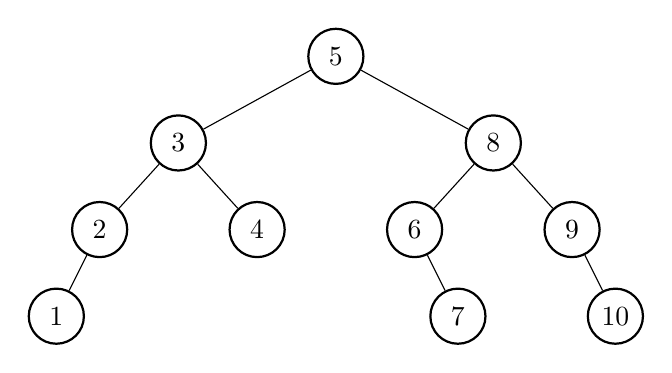
\begin{tikzpicture}[every node/.style={circle, draw, thick, minimum size=7mm, inner sep=0pt},
    level distance=11mm, level 1/.style={sibling distance=40mm}, level 2/.style={sibling distance=20mm},
    level 3/.style={sibling distance=11mm}]
\node {5}
  child {node {3}
    child {node {2} child {node {1}} child[missing]}
    child {node {4}}}
  child {node {8}
    child {node {6} child[missing] child {node {7}}}
    child {node {9} child[missing] child {node {10}}}};
\end{tikzpicture}
\end{center}

\textbf{(b)} 後序（左、右、根）：左子樹 $3$ 的部分是 $1, 2, 4, 3$；右子樹 $8$ 的部分是 $7, 6, 10, 9, 8$；最後是根。
\[
1,\ 2,\ 4,\ 3,\ 7,\ 6,\ 10,\ 9,\ 8,\ 5
\]

\textbf{(c)} $8$ 有兩個子節點，要用中序的前驅（左子樹最大的）或後繼（右子樹最小的）來取代它（資結書第~9.2~節），
兩種都對，所以有兩棵可能的樹：
\begin{itemize}
\item \textbf{用前驅 $7$}：左子樹 $\{6, 7\}$ 最大的是 $7$，$7$ 移到 $8$ 的位置，$7$ 原本是葉節點，直接拿掉。 $6$ 變成沒有子節點。
\item \textbf{用後繼 $9$}：右子樹 $\{9, 10\}$ 最小的是 $9$，$9$ 移到 $8$ 的位置，$9$ 原本的右子節點 $10$ 接到 $9$ 原本的位置。
\end{itemize}

\begin{center}
\begin{tikzpicture}[every node/.style={circle, draw, thick, minimum size=7mm, inner sep=0pt},
    level distance=10mm, level 1/.style={sibling distance=30mm}, level 2/.style={sibling distance=15mm},
    level 3/.style={sibling distance=9mm}, lab/.style={draw=none, rectangle, font=\small}]
\node {5}
  child {node {3}
    child {node {2} child {node {1}} child[missing]}
    child {node {4}}}
  child {node {7}
    child {node {6}}
    child {node {9} child[missing] child {node {10}}}};
\node[lab] at (0,-4.0) {用前驅 7 取代};
\begin{scope}[xshift=7.5cm]
\node {5}
  child {node {3}
    child {node {2} child {node {1}} child[missing]}
    child {node {4}}}
  child {node {9}
    child {node {6} child[missing] child {node {7}}}
    child {node {10}}};
\node[lab] at (0,-4.0) {用後繼 9 取代};
\end{scope}
\end{tikzpicture}
\end{center}

\textbf{(d)} 「Top-Down」是逐一插入：每個新數放在完全二元樹的下一個位置（陣列的尾端），再往上和父節點比，比父節點
小就交換，直到不比父節點小或到根（資結書第~8.1~節）。 陣列下標從 $1$ 開始，$i$ 的父節點是 $\lfloor i/2\rfloor$。

\begin{center}
\small
\begin{tabular}{rll}
\toprule
插入 & 往上調整 & 陣列 $A[1..]$ \\
\midrule
5 & & 5 \\
3 & $3 < 5$，換 & 3, 5 \\
8 & $8 > 3$，不動 & 3, 5, 8 \\
2 & 放在 4，$2 < 5$ 換到 2，$2 < 3$ 換到 1 & 2, 3, 8, 5 \\
6 & 放在 5，$6 > 3$，不動 & 2, 3, 8, 5, 6 \\
7 & 放在 6，$7 < 8$ 換到 3，$7 > 2$ 停 & 2, 3, 7, 5, 6, 8 \\
1 & 放在 7，$1 < 7$ 換到 3，$1 < 2$ 換到 1 & 1, 3, 2, 5, 6, 8, 7 \\
9 & 放在 8，$9 > 5$，不動 & 1, 3, 2, 5, 6, 8, 7, 9 \\
10 & 放在 9，$10 > 5$，不動 & 1, 3, 2, 5, 6, 8, 7, 9, 10 \\
4 & 放在 10，$4 < 6$ 換到 5，$4 > 3$ 停 & 1, 3, 2, 5, 4, 8, 7, 9, 10, 6 \\
\bottomrule
\end{tabular}
\end{center}

\begin{center}
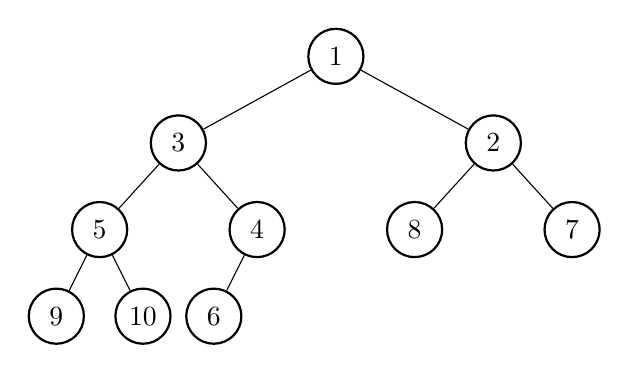
\begin{tikzpicture}[every node/.style={circle, draw, thick, minimum size=7mm, inner sep=0pt},
    level distance=11mm, level 1/.style={sibling distance=40mm}, level 2/.style={sibling distance=20mm},
    level 3/.style={sibling distance=11mm}]
\node {1}
  child {node {3}
    child {node {5} child {node {9}} child {node {10}}}
    child {node {4} child {node {6}} child[missing]}}
  child {node {2}
    child {node {8}}
    child {node {7}}};
\end{tikzpicture}
\end{center}

\textbf{(e)} 刪除最小值 $1$（根）：把最後一個 $A[10] = 6$ 移到根，堆積少一個，再從根往下調整：和比較小的子節點比，比它大就
交換（資結書第~8.1~節）。
\begin{itemize}
\item $6$ 在根，子節點 $3$、$2$，較小的是 $2$，$6 > 2$，交換：$2$ 上來，$6$ 到位置 3。
\item $6$ 在位置 3，子節點 $8$、$7$，較小的是 $7$，$6 < 7$，停。
\end{itemize}
結果陣列 $2, 3, 6, 5, 4, 8, 7, 9, 10$：
\begin{center}
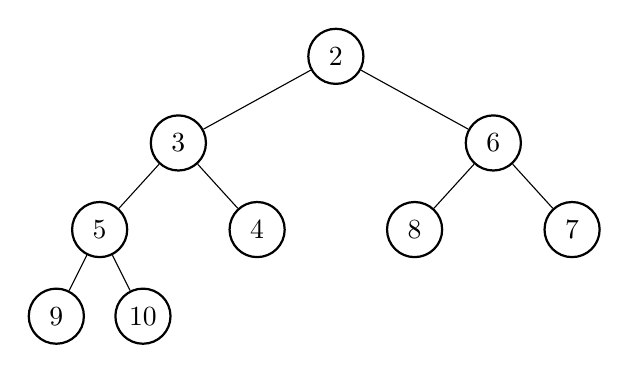
\begin{tikzpicture}[every node/.style={circle, draw, thick, minimum size=7mm, inner sep=0pt},
    level distance=11mm, level 1/.style={sibling distance=40mm}, level 2/.style={sibling distance=20mm},
    level 3/.style={sibling distance=11mm}]
\node {2}
  child {node {3}
    child {node {5} child {node {9}} child {node {10}}}
    child {node {4}}}
  child {node {6}
    child {node {8}}
    child {node {7}}};
\end{tikzpicture}
\end{center}
\end{pastsoln}
